\documentclass{article}

% Language setting
\usepackage[english]{babel}

% Set page size and margins
\usepackage[letterpaper,top=2cm,bottom=2cm,left=3cm,right=3cm,marginparwidth=1.75cm]{geometry}

% Useful packages
\usepackage{amsmath}
\usepackage{amssymb}
\usepackage{graphicx}
\usepackage{booktabs}
\usepackage{multirow}
\usepackage[colorlinks=true, allcolors=blue]{hyperref}
\usepackage[round]{natbib}

\title{Market Making via Reinforcement Learning Under Simulated Market Impact: A Queue-Reactive Reassessment of Spooner et al.}
\author{Dylan McClish}

\begin{document}
\maketitle

\begin{abstract}
Reinforcement Learning (RL) is a powerful tool that has much potential in the financial markets. In Spooner et al.'s Market Making via Reinforcement Learning, varying configurations of RL agents are trained and evaluated on historical order book data. However, this historical order book does not allow for market impact, nor is it easily generalizable for robust testing. To address this, we investigate the RL agent configuration of Spooner in a simulated order-book environment. We use a Zero-Intelligence model as a control, and then a Queue-Reactive model as a more realistic environment with market impact. The total PnL, mean absolute position, and trading behavior of the agents is then evaluated. In the Queue-Reactive simulator, the basic agent is essentially inactive (0.0 fills/episode) while the consolidated agent trades meaningfully more (33.0 fills/episode) yet still keeps its mean absolute position near zero (0.01, versus 0.00 for the basic agent). This suggests that, even under simulated market impact, the consolidated agent's richer state representation lets it trade far more actively than the basic agent while still keeping its own inventory close to zero, echoing the inventory-management advantage Spooner reports for the historical order book.


\end{abstract}

\section{Introduction}

Reinforcement learning is a popular approach to have machines learn. Like a dog who learns to sit through command and presence of a treat, an agent can mathematically learn the optimal policy through the reward it receives for a given action from a given scenario \citep{suttonbarto2018}. As many novel technologies have, there are, of course, applications in finance. In trading, one of the most prominent strategies is market making (MM) where "market makers" place quotes around a fair value. If the fair value changes while market makers have a net position, then market makers will make or lose money from their positions. This is considered a principal risk of prototypical market makers as they do not know the direction that fair value may move. The optimal manner to maximize returns while minimizing risk of market makers is an existing problem. In Spooner's \textit{Market Making via Reinforcement Learning}, he develops a RL MM agent that exhibits superior returns compared to the prior benchmark \citep{spooner2018}. In simulating the environment to train the RL agents, he uses real order book data and argues that this is the most realistic form to represent historical data. However, there are multiple issues with the usage of historical data, but principally, it can't represent market impact of an agent and is limited in availability. I use Spooner's framework to train an agent on a simulated order book environment. In turn, we can analyze how his results differentiate between alternate order book environments. Using a simulated order book allows us to also precisely understand the generating mechanism of the order book, which aids in our discussion of the results.

Instead of historical data, I utilize the Queue-Reactive model developed by Huang \citep{huang2015}, which is a model of the order book that changes behavior based on the amount of resting quotes in the market. This represents more realistic assumptions of order book behavior, while allowing us to analyze how the agents analyzed by Spooner behave under market impact.

\section{Background}

\subsection{Reinforcement Learning}

First, we briefly discuss reinforcement learning. We use the description of the multi-armed bandit found in Sutton and Barto \citep{suttonbarto2018}. For simplicity, we only consider infinite-horizon problems that have no terminating state.

The foundation of RL is best described through the multi-armed bandit problem. Suppose we had multiple slot machines each of which has a different distribution of rewards associated with it that is unknown to us. We can take an action to use one of the slot machines, and we directly observe the reward attained from doing so. The natural question is how can we attain the most rewards from these slot machines?

Clearly, this problem involves finding the slot machine with the largest expected reward and then maximally exploiting this slot machine. However, we need to attain accurate estimates of the expected reward of the slot machines. This requires adequate samples from each slot machine. This can be done with the following formula \citep{suttonbarto2018}:
\begin{equation}
Q_t(a) = \frac{\sum_{i=1}^{t-1} R_i \cdot \mathbb{1}_{A_i = a}}{\sum_{i=1}^{t-1} \mathbb{1}_{A_i = a}},
\end{equation}
where $A_i$ and $R_i$ are the action taken and reward received at step $i$, and $Q_t(a)$ is our estimate, at step $t$, of the expected reward of slot machine $a$.

There is also an incremental update version of this formula that is more space-efficient, since it does not require storing every past reward:
\begin{equation}
Q_{n+1} = Q_n + \frac{1}{n}\left[R_n - Q_n\right].
\end{equation}

There are many approaches to solving this. Crudely, we would engage in a large degree of initial exploration as we figure out our estimates for the slot machines, then we would gradually decrease this exploration and begin to exploit our estimates by choosing the slot machine with the largest estimated expected reward.

Now imagine that we have multiple labeled rooms full of these slot machines. The slot machines are identical in each room, however they have different reward distributions. In each turn, we are randomly placed in one of these rooms. Based on the room labeling, we know which room we are in on any given turn. To solve this problem, we do a very similar process to above. However, we must keep track of multiple estimates of the slot machines based on the room that we are currently in, i.e., we estimate $Q_t(s,a)$ for each room $s$ separately.

Finally, now instead of being randomly placed in each room, the room that you are placed in is based off the slot machine that you chose in a given room. The estimates of the value of each slot machine in each room now depends on not only the immediate reward given by the slot machines but also how they transition you to different rooms. To account for this, we must change how we estimate the expected value of these machines. We can make each sample of this expected value the immediate reward that we get plus the expected value of the new room that we transition to, which we can define as the maximum of the expected reward of all the slot machines in this room. We can discount the expected reward of all the slot machines by some factor $0 < \gamma < 1$ in order to introduce natural human intuition of temporal discounting.

This looks like the following:
\begin{equation}
Q(s,a) \leftarrow Q(s,a) + \alpha\Big[R + \gamma \max_{a'} Q(s',a') - Q(s,a)\Big],
\end{equation}
where $s'$ is the room we land in after choosing slot machine $a$ in room $s$, and $\alpha$ is a step-size (learning rate) parameter.


As evidenced, this is a recursive problem. We are constructing new estimates of long-run expected values of choosing a slot machine in a given room using old estimates of long-run expected values. It is a result of stochastic approximation theory, under standard step-size conditions, that these estimates still converge to the accurate long-run expected value \citep{suttonbarto2018}.

There are many approaches to solve this problem, along with natural extensions to the problem that make it increasingly complicated. However, this thought experiment serves as the foundation for a lot of reinforcement learning.

We can think of the room of the slot machines as our ``state,'' the slot machine that we choose as our ``action,'' and the reward that we get as our, big surprise here, ``reward.'' There are a surprising amount of problems that can be concisely represented using this framework. Mathematically, this framework is called the Markov Decision Process (MDP).

Given an MDP where we precisely know the reward function and how we transition between states, we can iteratively compute the optimal solution without interacting with the environment -- these are dynamic programming approaches. However, most realistic environments don't provide such information. The problem in RL is how we optimally sample from the environment itself to generate estimates of these long-run expected values of actions. Then, these long-run expected values allow us to generate a decision-making strategy or ``policy'' that allows us to exploit these estimates. There are a range of approaches to solving this problem which are outside the scope of this paper.

\subsection{Market Making}

In trading a given instrument, there is a fair value. Liquidity takers are market participants who are willing to buy at lower than the fair value or sell at higher than the fair value in order to instantly trade. There are liquidity providers, or market makers, who are providing resting buy quotes lower than the fair value and resting sell quotes higher than the fair value that the liquidity takers can instantly trade with.

Because the liquidity providers are providing resting quotes, they are getting compensated when a liquidity taker places an order at their quote. However, they have to ``pay'' in the sense that they don't get to trade immediately. If someone trades against the market maker who is aware of a change in fair value before the market maker, then the market maker risks accumulating inventory that will cause them to lose money if the market moves against them. In addition, the closer that the market maker provides quotes to the fair value, the more fills they get as liquidity takers are paying up less. However, this also means the market maker is compensated less.

This is the game played by market makers. There are many ways to address this problem.

For example, \citet{avellaneda2008} detail a procedural approach based on stochastic optimal control, but RL offers a modular, interpretable approach that allows us not only to replicate human behavior but also perhaps gain insight on novel approaches learned by the agent.

\section{Method}

\subsection{Overview}

In Spooner's paper, the consolidated agent outperforms the basic agent in the historical order book environment \citep{spooner2018}.

The main research question explored here is: does the consolidated agent retain this advantage over the basic agent in an order-book environment with market impact? This is examined through the performance of the consolidated and basic agent under a Zero-Intelligence, no-market-impact model to act as the control, and a Queue-Reactive market-impact model to act as the experimental group.

\subsection{Data and Calibration}

We sourced our data from IEX DEEP, a free, public real-time market data feed from the IEX exchange. It broadcasts full order-book depth plus trade prints. We collected it for INTC over 7 trading days. We parsed two record types out of the raw feed: price-level updates (add/update/delete at a given price and side) and trade reports (executed size/price). We reconstructed the book from the price-level stream and used the trade records to differentiate executed size from order cancellation. Then, we used these streams to calibrate our QR and ZI models (Section~\ref{sec:simulator}).

Similar to Spooner, we encountered the problem of having to differentiate between order cancellations and order execution from the IEX fed. Spooner addresses this through assuming order cancellations are uniformly distributed. However, we cross-reference the trade-report stream: a size decrease at a price with a same-price, near-simultaneous trade report (within a $2\,\mu s$ tolerance window) is attributed to an execution; otherwise it is attributed to a cancellation. This increases the realism of our parameters.

We reconstruct only the touch (best bid/ask, level 1) this way, walking the price-level-update stream in time order and tracking, for each touch-price update, the pre-event queue size and the time elapsed since the touch last changed. Levels 2--5 in the Queue-Reactive simulator reuse the same level-independent intensity functions fit at level 1 (Section~\ref{sec:simulator}). Each of the 7 trading days is reconstructed independently and the resulting limit-order-arrival and cancellation observations are pooled directly across days, while the market-order rate is estimated from the sum of each day's own (event count, time span).

IEX represents a small share of total US equity volume: approximately 3.8\% overall (4.7\% intraday-only) as of Q2 2026 \citep{iexmarketshare2026}, and it skews toward less-latency-sensitive flow because of its deliberate speed-bump design.

Though, it should be noted that this problem isn't unique to IEX. As of Q1 2026, dark pool volume alone reached 40.3\% of all US equity volume, and total off-exchange volume -- dark pools plus wholesaler internalization combined -- accounted for roughly 59\%, leaving only about 41\% occurring on lit exchanges \citep{tradealgo2026}. So even the primary listing exchange for a given stock does not see the full picture of order flow. We revisit the consequences of this for external validity in the Limitations discussion (Section~\ref{sec:limitations}).

\subsection{Simulator}
\label{sec:simulator}

We describe the two simulators used to generate data to train the models.

First, we have a Zero-Intelligence (ZI) simulator modeled after the Poisson model of Smith, Farmer, Gillemot, \& Krishnamurthy \citep{smith2003}. This model generates an order book using independent Poisson processes to simulate the market, limit, and cancellation orders. These processes have constant rates, independent of the current queue state. When limit orders arrive, they are randomly placed uniformly on a quote.

Next, we have a Queue-Reactive (QR) simulator from Huang \citep{huang2015}. Given a fixed reference price, this simulator models the limit order book as a vector of Poisson processes at each level relative to the reference price. The rate of the Poisson process is dependent on the current resting volume at that given level. The rates are estimated by collecting samples from a live order book. For each level and queue size, there are three different Poisson processes that represent market, limit, and cancel orders.

Then, the QR simulator allows the reference price to change. This happens mechanically with a probability $\theta$ when the mid price changes. The mid price can change simply through mechanical order book dynamics. When the reference price changes, the simulator will either (1) simply adjust all quotes to that of its neighbor (if the reference price increases, all levels will change to the value of the level above) or (2) with probability $\theta_{\text{init}}$ the LOB will completely reinitialize from the steady state distribution. $\theta_{\text{init}}$ represents the behavior of the LOB in reshuffling based on the injection of exogenous information, like market-moving news.

Namely, Huang demonstrates that this model mimics key market properties. For example, it illustrates the tendency for market participants to be less aggressive with limit orders when the top of book is sparse in available liquidity. A complete illustration of these properties can be found in Huang \citep{huang2015}, pp.\ 8--9.

\subsection{Agent Architecture}

We analyze the behavior of the basic and consolidated agent developed by Spooner \citep{spooner2018}.

The purpose of the basic agent is to construct a lower bound for the performance of the agent in this new market environment. The basic agent has the following configuration:

\begin{itemize}
  \item \textbf{State}: only known states are internal to the agent. In Spooner, this is current inventory and normalized bid/ask quoting distances ($\theta_a$, $\theta_b$).
  \item \textbf{Reward}: simple, undamped PnL. Following each event, the markout PnL is
    \begin{equation}
    r_t = \psi_t = \psi_t^{a} + \psi_t^{b} + I_t \cdot \Delta m_t,
    \end{equation}
    where $\psi_t^{a} = q_t^{a}(p_t^{a} - m_t)$ if the agent's ask was filled that step (0 otherwise), $\psi_t^{b} = q_t^{b}(m_t - p_t^{b})$ if the agent's bid was filled, $I_t$ is the agent's current inventory, and $\Delta m_t$ is the change in mid-price over the step \citep{spooner2018}.
  \item \textbf{Learning}: SARSA($\lambda$) with replacing eligibility traces.
\end{itemize}

Then, we use the ``consolidated agent'' of Spooner. This agent utilizes the optimal configuration amongst those explored by Spooner. We will compare this consolidated agent to the basic agent under our market simulator to analyze if there is a similar pattern of effects to that of Spooner. The consolidated agent has the following configuration:

\begin{itemize}
  \item \textbf{State}: three independent tile codings encode the state -- one tile-coding group is just agent variables, one is just market variables, and another is all of them combined (Table~\ref{tab:state-vars}). These tile codings are then consolidated via fixed weights,
    \begin{equation}
    \hat{Q}(s,a) = 0.6\,\hat{Q}_{\text{agent}}(s,a) + 0.1\,\hat{Q}_{\text{market}}(s,a) + 0.3\,\hat{Q}_{\text{full}}(s,a).
    \end{equation}
    (The basic agent above is the degenerate case that uses only the agent-group tiling, with weight 1.)
  \item \textbf{Reward}: an ``asymmetrically-dampened PnL.'' This is a PnL function that, in addition to the realized PnL from traders crossing the MM quotes, also penalizes unrealized losses from inventory while ignoring unrealized gains from inventory:
    \begin{equation}
    r_t = \psi_t - \max\big(0,\ \eta \cdot I_t \cdot \Delta m_t\big), \qquad \eta = 0.6.
    \end{equation}
    This is designed to mimic realistic MM behavior where market makers do not want to accumulate inventory. This is because they are intrinsically not making predictions on the direction of the fair price, so any unrealized gains from their inventory are not due to their knowledgeable trading. Thus, they can be attributed to luck.
  \item \textbf{Learning}: SARSA($\lambda$) with replacing eligibility traces. Note this is designed to be identical to the basic agent -- only the state representation and reward function change.
\end{itemize}

Tile codings are a method to discretize continuous state spaces through multiple offsetting buckets. In a simple discretization of a continuous space, points that are very close to each other may fall in separate buckets. If encoded as entirely separate states, the algorithm will treat them as such. However, tile codings use multiple offsetting buckets to allow points that fall close to each other in the original space to still potentially fall in the same bucket in a given set of buckets. Thus, this allows a more complete representation of the original space \citep{suttonbarto2018}.

\begin{table}[h]
\centering
\caption{State variables for the consolidated agent's three tile-coding groups.}
\label{tab:state-vars}
\begin{tabular}{@{}lll@{}}
\toprule
Group & \# vars & Variables \\
\midrule
Agent-state  & 3 & inventory, $\theta_a$, $\theta_b$ (normalized) \\
Market-state & 6 & spread, mid-price move, imbalance, signed volume, volatility, RSI \\
Full-state   & 9 & concatenation of the agent- and market-state variables \\
\bottomrule
\end{tabular}
\end{table}

\begin{table}[h]
\centering
\caption{Shared hyperparameters for both agents (Section~\ref{sec:exp-design} notes where we deviate from Spooner's Table 2 values).}
\label{tab:hyperparams}
\begin{tabular}{@{}ll@{}}
\toprule
Parameter & Value \\
\midrule
Memory size (tile-coding hash table) & $10^{7}$ \\
Tilings ($M$) & 32 \\
Tiles per dimension & 8 \\
LCTC group weights [agent, market, full] & $(0.6,\ 0.1,\ 0.3)$ \\
Learning rate $\alpha$ & 0.001 \\
Discount $\gamma$ & 0.97 \\
Trace parameter $\lambda$ & 0.96 \\
Exploration $\varepsilon_{\text{init}}$ / floor / $T$ & $0.7\ /\ 0.0001\ /\ 1000$ \\
Order size $\omega$ & 1000 \\
Inventory bounds & $[-10000,\ 10000]$ \\
\bottomrule
\end{tabular}
\end{table}

\subsection{Experimental Design}
\label{sec:exp-design}

To construct our experiment, we construct 4 training scenarios that consist of each agent architecture trained and tested in each simulator environment (Table~\ref{tab:grid}).

\begin{table}[h]
\centering
\caption{The $2\times2$ experimental grid: agent architecture $\times$ simulator, all four cells trained on a matched budget of 400 episodes ($\varepsilon_t = 400$). A fifth, bonus run -- the consolidated agent under QR at Spooner's original 1000-episode budget ($\varepsilon_t = 1000$) -- is kept outside the core comparison as a robustness check, since it is not on the same training budget as the other four cells.}
\label{tab:grid}
\begin{tabular}{@{}lcc@{}}
\toprule
 & ZI simulator (control) & QR simulator (market impact) \\
\midrule
Basic agent        & 400 episodes & 400 episodes \\
Consolidated agent & 400 episodes & 400 episodes \\[2pt]
\multicolumn{3}{@{}l}{\footnotesize \textit{Bonus (outside core grid):} Consolidated agent, QR, 1000 episodes} \\
\bottomrule
\end{tabular}
\end{table}

We resemble Spooner's experimental design. However, we deviate in a few crucial ways.

For one, we use 400 training episodes instead of 1000, due to computing constraints. We rescale the epsilon-schedule to attain an equivalent exploration trajectory in this shortened training time: setting $\varepsilon_t = 400$ reproduces the identical epsilon trajectory that Spooner's $\varepsilon_t = 1000$ schedule would trace out over the full 1000 episodes, just compressed into 400 episodes ($\varepsilon(400;\varepsilon_t{=}400) = \varepsilon(1000;\varepsilon_t{=}1000) = 0.350$). This was done due to computing limitations, though the agents still displayed meaningful convergence in this shortened training time. All four cells of the grid are trained on the same 400-episode budget so that the basic-vs-consolidated and ZI-vs-QR comparisons are not confounded by unequal training exposure.

Second, we use simulation to generate data for the agents rather than utilize historical data. Historical data is not always easy or cheap to attain, so simulators play a crucial role in developing models. We use this experiment to investigate a few key questions:
\begin{enumerate}
  \item Do Spooner's agents still demonstrate the same relative performance in this new market environment?
  \item How does the strategy of Spooner's agents differ between the Zero-Intelligence environment and the Queue-Reactive environment (which has market impact)?
\end{enumerate}

\subsection{Evaluation}

To evaluate the models, we took the $\varepsilon$-greedy strategy with $\varepsilon = 0$ to remove exploration noise. The $\varepsilon$-greedy agent-environment configuration is then compared to multiple benchmark policies: fixed-spread market makers that hold a symmetric quote ($\theta_a = \theta_b = \theta$, for $\theta \in \{1,\dots,5\}$) for the entire episode, and a random agent that performs a uniformly-random action every event. All policies are run through identical simulator environments, using the same underlying environment mechanics as training (fill resolution, inventory bounds).

The metrics that we used were the following:
\begin{enumerate}
  \item \textbf{Normalized daily PnL}: (final cash + inventory $\times$ final mid-price) / number of events in episode, averaged over episodes with standard deviation reported.
  \item \textbf{Mean absolute position (MAP)}: the time-average of $|\text{inventory}|$ across the whole episode, averaged across all episodes.
\end{enumerate}

The testing window was an episode consisting of 5{,}000{,}000 events drawn from the simulator, averaged over 5 episodes per policy (using seeds disjoint from training). This is approximately $\tfrac{1}{3}$ of a training day at the rate of events estimated from the IEX data ($17{,}600{,}000$ events/day; see Limitations, Section~\ref{sec:limitations}, for the consequences of this mismatch).

\subsection{Computational Implementation}

The entire implementation can be found at \url{https://github.com/dylanmcclish/rl-market-making-qr-impact}.

\section{Results}
\label{sec:results}

An overview of the results of each RL agent and the benchmarks is shown in Table~\ref{tab:results}, and the corresponding fill counts, averaged over the same 5 episodes $\times$ 5{,}000{,}000 events, in Table~\ref{tab:fills}.

\begin{table}[h]
\centering
\caption{Normalized daily PnL and mean absolute position (MAP) for the greedy ($\varepsilon=0$) trained agents and the fixed-spread/random benchmarks, evaluated over 5 episodes $\times$ 5{,}000{,}000 events. Std.\ dev.\ is across the 5 episodes.}
\label{tab:results}
\small
\begin{tabular}{@{}lrrrr@{}}
\toprule
 & \multicolumn{2}{c}{QR simulator} & \multicolumn{2}{c}{ZI simulator} \\
\cmidrule(lr){2-3}\cmidrule(lr){4-5}
Policy & Norm.\ PnL (std) & MAP & Norm.\ PnL (std) & MAP \\
\midrule
Basic agent (greedy)          & 0.000000 (0.000000) & 0.00    & 0.000002 (0.000001) & 98.74 \\
Consolidated (greedy, 400ep)  & $-$0.000013 (0.000006) & 0.01    & 0.000001 (0.000002) & 35.33 \\
Consolidated (greedy, 1000ep, bonus) & $-$0.000056 (0.000050) & 0.01 & --- & --- \\
Fixed $\theta=1$               & 2.225312 (0.092453) & 3398.78 & 0.000156 (0.000012) & 628.08 \\
Fixed $\theta=2$               & 0.000000 (0.000000) & 0.00    & 0.000005 (0.000001) & 67.26 \\
Fixed $\theta=3$               & 0.000000 (0.000000) & 0.00    & 0.000000 (0.000001) & 19.18 \\
Fixed $\theta=4$               & 0.000000 (0.000000) & 0.00    & 0.000001 (0.000001) & 11.29 \\
Fixed $\theta=5$               & 0.000000 (0.000000) & 0.00    & 0.000000 (0.000000) & 0.00 \\
Random                         & $-$0.000023 (0.000014) & 0.01    & $-$0.000000 (0.000000) & 0.00 \\
\bottomrule
\end{tabular}
\normalsize
\end{table}

\begin{table}[h]
\centering
\caption{Fill counts (mean $\pm$ std.\ dev.) over the same 5 episodes $\times$ 5{,}000{,}000 events, and the same 5 seeds, as Table~\ref{tab:results} -- reported separately since \texttt{eval.cpp} itself only aggregates PnL/MAP; these come from a companion diagnostic run against the same trained weights and benchmark policies.}
\label{tab:fills}
\small
\begin{tabular}{@{}lrr@{}}
\toprule
Policy & QR fills & ZI fills \\
\midrule
Basic agent                  & 0.0 $\pm$ 0.0    & 1.2 $\pm$ 1.0  \\
Consolidated agent (400ep)   & 33.0 $\pm$ 7.8   & 2.8 $\pm$ 2.3  \\
Consolidated agent (1000ep, bonus) & 27.4 $\pm$ 2.8 & --- \\
Fixed $\theta=1$              & 1400.8 $\pm$ 17.1 & 225.4 $\pm$ 9.2 \\
Fixed $\theta=2$              & 0.2 $\pm$ 0.4    & 1.8 $\pm$ 1.6  \\
Fixed $\theta=3$              & 0.0 $\pm$ 0.0    & 0.4 $\pm$ 0.5  \\
Fixed $\theta=4$              & 0.0 $\pm$ 0.0    & 0.0 $\pm$ 0.0  \\
Fixed $\theta=5$              & 0.0 $\pm$ 0.0    & 0.0 $\pm$ 0.0  \\
Random                        & 31.6 $\pm$ 5.9   & 1.6 $\pm$ 1.2  \\
\bottomrule
\end{tabular}
\normalsize
\end{table}

These results are discussed in Section~\ref{sec:discussion}.

\begin{figure}[h]
\centering
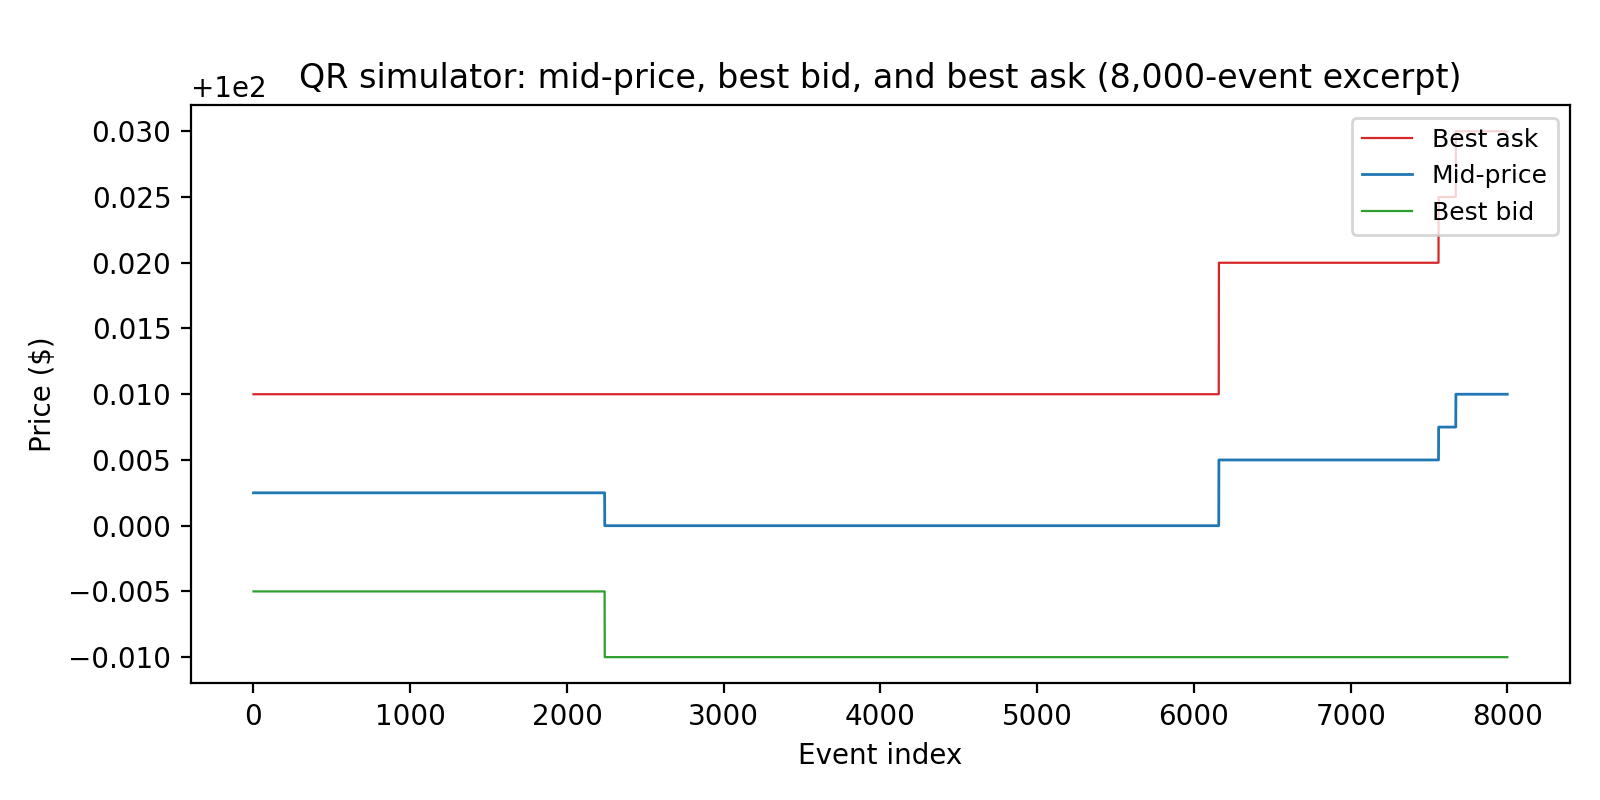
\includegraphics[width=0.8\textwidth]{figures/market_environment_timeseries.png}
\caption{Mid-price, best bid, and best ask over an 8,000-event excerpt of the QR simulator (not the full 5,000,000-event evaluation episode, which is illegible as a line plot at that scale).}
\label{fig:market-env}
\end{figure}

\section{Discussion}
\label{sec:discussion}

Interestingly, the consolidated agent performs slightly worse than the basic agent in the testing set in both simulators. Both agents perform markedly worse in PnL than the fixed $\theta=1$ benchmark (2.225 compared to 0 and $-0.000013$).

However, the $\theta=1$ benchmark has a MAP of 3398.78 in the QR simulator and 628.08 in the ZI simulator. This reflects the lack of penalty on inventory of the fixed agent. This lack of inventory management indicates that $\theta=1$ was exposed to large amounts of inventory risk during the testing episode. Although this turned out in its favor, this is a fixed-width policy with no knowledge of the market environment. If a large swing happened in the price due to some fundamental change in the market, the fixed-width agent would accumulate a large inventory position at increasingly worse prices.

Interestingly, while actively trading, the consolidated agent is effectively managing the MAP, with a value of 0.01. Though it should be noted that the consolidated agent averages only 33.0 fills in the QR simulator and 2.8 in the ZI simulator over a 5{,}000{,}000-event episode (Table~\ref{tab:fills}), compared to means of 1400.8 (QR) and 225.4 (ZI) for the $\theta=1$ benchmark.

Next, in the QR environment, the basic agent learns to never trade (0.0 fills in Table~\ref{tab:fills}); in the ZI environment it trades only exceedingly rarely (a mean of 1.2 fills per 5{,}000{,}000-event episode). I hypothesize that this is a result of the configuration of the basic agent in conjunction with the market environment. In this market, fills are very sparse. So, most actions taken by an agent are going to be viewed as having essentially zero reward. Moreover, the basic agent only has access to internal state information (current active quotes and inventory). So, the lack of information of the agent on the market state means that it is likely not getting consistently advantageous fills. Thus, the rewards are likely negative or indistinguishable from zero, and the agent converges on almost never trading as a consequence.

However, the relative comparison on inventory management between the basic agent and the consolidated agent is most interesting. As Spooner observes, ``the basic agent regularly holds a non-zero inventory, exposing itself to changes in the security's value for extended periods of time\ldots [while] for the consolidated agent, it appears that the learnt policy targets a near-zero inventory, relying less on speculative trading and thus yielding the consistency one expects from a good market making strategy'' \citep{spooner2018}. The statistics reveal that the basic agent and consolidated agent in this simulated environment exhibit very similar results. The MAP can be viewed as a proxy for the absolute mean of the inventory process. The MAP of the basic agent was 0 in the QR environment and 98.74 in the ZI environment. The MAP of the consolidated agent was 0.01 in the QR environment and 35.33 in the ZI environment. It is interesting that the consolidated agent better effectively managed position within the market-impact QR environment. Coupled with the average of 33.0 fills/episode of the consolidated agent, this suggests that the more realistic market dynamics were leveraged by the consolidated agent to reduce inventory.

\subsection{Limitations}
\label{sec:limitations}

The simulators were calibrated on data from the IEX. This was done due to data accessibility. However, IEX only represents about 3.8--4.7\% of all US equity trading volume \citep{iexmarketshare2026} and typically attracts low-latency-averse traders since it was designed to deter HFT flow (its signature ``speed bump''). This may explain the sparse fills observed in our results, but it also means that we are not representing a substantial amount of the flow that would be seen on the primary listing exchange or in off-exchange venues, which together account for the majority of total volume \citep{tradealgo2026}.

The testing window used was not a full training day: our 5{,}000{,}000-event evaluation window is roughly 28\% of the 17{,}600{,}000-event training episode length.

\section{Future Research}

One of the directions that I find most interesting is the analysis of RL on order flows from dark pools. Dark pools are designed to hide resting order activity to limit price impact from large flow. However, roughly 59\% of total US equity volume trades off-exchange -- dark pools plus wholesaler internalization combined \citep{tradealgo2026} -- so it is definitely a source of interest for major institutional investors. This would require a model of dark pool order dynamics and a thorough understanding of its relationship to lit exchanges. However, this introduces difficulty due to the natural lack of data available from dark pools.

It would also be interesting to analyze an RL algorithm using an online learning approach. This would allow us to directly see how the agent evolves under changing market conditions.


\bibliographystyle{plainnat}
\bibliography{sample}

\end{document}
